
\documentclass[a4paper, 9pt]{proc} % Font size (can be 10pt, 11pt or 12pt) and paper size (remove a4paper for US letter paper)

% \usepackage[protrusion=true,expansion=true]{microtype} % Better typography
\usepackage{graphicx} % Required for including pictures
\usepackage{wrapfig} % Allows in-line images
\usepackage{gensymb}

\usepackage[font={small,it}]{caption}
\usepackage[font={scriptsize,it}]{subcaption}

% \captionsetup{justification=centering}

\usepackage{mathpazo} % Use the Palatino font
\usepackage[T1]{fontenc} % Required for accented characters
\linespread{1.0} % Change line spacing here, Palatino benefits from a slight increase by default

\makeatletter
% \renewcommand\@biblabel[1]{\textbf{#1.}} % Change the square brackets for each bibliography item from '[1]' to '1.'
% \renewcommand{\@listI}{\itemsep=0pt} % Reduce the space between items in the itemize and enumerate environments and the bibliography

\renewcommand{\maketitle}{ % Customize the title - do not edit title and author name here, see the TITLE block below
\begin{centering} % Right align
{\huge\@title} % Increase the font size of the title

\vspace{20pt} % Some vertical space between the title and author name

{\large\@author} % Author name
%\\\@date % Date

\vspace{10pt} % Some vertical space between the author block and abstract
\end{centering}
}

%----------------------------------------------------------------------------------------
%	TITLE
%----------------------------------------------------------------------------------------

\title{\textbf{Deep Cuts}\\ % Title
\Large{shot detection for cinematographic analysis}} % Subtitle

\author{\textsc{Rachel Albert\\ Alex Hall\\ Jonathan Harper\\ Amy Pavel} % Author
\\{\textit{\\CS280 Final Project, Spring 2015}}} % Institution


%\date{\today} % Date

%----------------------------------------------------------------------------------------

\begin{document}

\maketitle % Print the title section

%----------------------------------------------------------------------------------------
%	ABSTRACT AND KEYWORDS
%----------------------------------------------------------------------------------------

%\renewcommand{\abstractname}{Summary} % Uncomment to change the name of the abstract to something else

%\begin{abstract}
%Text goes here
%\end{abstract}
%
%\hspace*{3,6mm}\textit{Keywords:} lorem , ipsum , dolor , sit amet , lectus % Keywords
%
%\vspace{30pt} % Some vertical space between the abstract and first section

%----------------------------------------------------------------------------------------
%	ESSAY BODY
%----------------------------------------------------------------------------------------

\section*{Introduction}

Much like authors and editors of written language, cinematographers and film editors have their own unique style.
Modern cinematographers use a well-defined visual language to create motion-pictures. Our goal is to better understand the use of cinematographic techniques in defining a motion-picture's visual style. What types of shots are most common? Are certain shots arranged in predictable ways across many motion-pictures?

In this work we focus on automatically classifying frame composition and sequential structure in film.  To do so we first classify the composition of individual frames based on the number of actors and placement of each actor in the frame.  We then analyze the the sequential structure of a film by mining patterns in the frame classes determined in the previous step.  The classes and sequential structures recovered during this process closely match with the terminology used by professional cinematographers~\cite{arijon_grammar_1991}.  

We finally recognize that we can better understand film composition by also recognizing a film's shots (transitions from one camera to another), and we implement two state-of-the-art approaches for camera shot boundary detection.

%%% Local Variables:
%%% mode: latex
%%% TeX-master: "finalpaper"
%%% End:


\section*{Background \& Significance}

Literature review and short summary of our contribution goes here.

\section*{Composition and Face Detection}

We analyze film composition at two levels of abstraction: the \emph{frame} and the \emph{sequence}.  A frame is a single image produced by a camera in the film.  A sequence is a series of camera shots, where each shot is an unbroken series of frames produced by a single camera.  Frame composition and sequence structure provide a sufficient basis upon which to begin analysis, are explicitly defined, and are directly related to the work of the cinematographer.

To analyze frame composition and sequence structure we first classify each frame and then use patterns in the sequence of frame classes to determine sequential structure.

\subsection*{Frame Composition}

We restrict our description of the frame composition to population, zoom and position of actors in the frame. Other visual elements, such as non-human points of interest (e.g. a car in the midst of a chase sequence) can be as or more important than actors in a given frame; however, actors are at the core of most motion-pictures, and are therefore a good point of entry for better automatic understanding frame composition. To detect the population, zoom and position of actors in each frame we use a state-of-the-art face detector~\cite{mathias_face_2014}.

The population of a frame is defined as the number of faces visible. We consider a face to be valid whether it is an actor, a photograph, a movie-within-a-movie or some other indirect face. A face is also valid regardless of minor occlusions (e.g. hair or partial masks) and orientation (e.g. face is oriented away from the camera). A face is invalid if it is non-human (e.g. animals, monsters, drawings, or CGI renderings). 

Zoom is the perceived distance between camera and actor. This is typically classified by how much of the actor is visible within the shot. Figure \ref{fig:zoomClass} shows the seven commonly used zoom classifications. We stick to the traditional nomenclature of ``shot'', though we are classifying frames. The classifications  are, in descending order of ``closeness'':


%%%%%%%%%%%%%%%%%%%%%%%%%%%%%%

\textbf{Extreme Close-Up - ECU} The camera is so close to the actor that the actor's face exceeds the size of the frame.

\textbf{Close-Up - CU} The viewer can see the actor's entire face, but the shoulders are typically not in the frame. 

\textbf{Medium Close-Up - MCU} These frames contain the actor's entire face as well as their neck, shoulders, and clavicular region. 

\textbf{Medium Shot - MS} These frames show the actor from the abdomen and above. 

\textbf{Medium Long Shot - MLS} These frames contain most, but not all of an actor's body. The shots typically contain some or all of the leg, but will not show the feet. %A common location to cut-off the actor in these shots is at the knees. Cutting at mid-thigh, the knees, or mid-shin is considered more visually appealing than cutting at the ankles \cite{arijon_grammar_1991}.

\textbf{Long Shot - LS} The actor's entire body, from head to toe, is visible. In these frames, the actor is generally still in the forefront of the frame. 

\textbf{Extreme Long Shot - ELS} In these shots, the actor is visible, but at a significant distance from the camera. 

%%%%%%%%%%%%%%%%%%%%%%%%%%%%%%

We assume that the proportion between the height of an actor's head and the height of their body is relatively consistent across actors. We define the 7 types of zoom by the ratio of the face height, $f$, to the frame height, $h$. By taking measurements of pre-classified frames, we computed the following $f$:$h$ ratios for each class of zoom:

%%%%%%%%%%%%%%%%%%%%%%%%%%%%%%
\begin{center}
  \small{
  \begin{tabular}{ l | l l}
    Shot Name & Abbrv. & Range \\ \hline
    Extreme Close-Up & ECU & $f > h$ \\ 
    Close-Up & CU & $h \geq f > 0.6h$ \\ 
    Medium Close-Up & MCU & $0.6h \geq f > 0.3h$ \\ 
    Medium Shot & MS & $0.3h \geq f > 0.2h$ \\ 
    Medium Long Shot & MLS & $0.2h \geq f > 0.1h$ \\ 
    Long Shot & LS & $0.1h \geq f > 0.02h$ \\ 
    Extreme Long Shot & ELS & $0.02h \geq f$
    \label{tab:zoomTypes}
  \end{tabular}
  }
\end{center}
%%%%%%%%%%%%%%%%%%%%%%%%%%%%%%

These ratios are applied to the bounding boxes produced by face detectors. The height of the bounding box our $f$ and the vertical resolution of the frame our $h$. Note that in the case of frames with population $> 1$, we tag the frame based on the face closest to the camera. 

%--------------------------------------------------------------------------------
\subsubsection*{Positioning}
Frame composition is also defined by the position of faces in the frame. Texts on cinematography frequently divide a frame horizontally into 2, 3, or 4 parts and vertically into 2 or 3 parts. We divide the frame into a $3\times 3$ grid. The vertical classifications are top, middle, \& bottom. The horizontal classifications are left, center, \& right. These classifications are considered in isolation or combinatorially to create, for example, top-right and middle-center. This classification has the advantage of clear perceptual salience. While it is difficult to discern whether a face is in the left quarter of a frame compared to the left third of a frame, it is much easier to determine whether it is centered, in the left third, or in the right third. Edge cases, such as frames composed using the `rule of thirds', are difficult for a human to classify; however, the $3\times 3$ grid offers a good compromise between precision and visual salience. A frame is given a tag corresponding to the grid cell containing the centroid of the largest face in the frame. Figure \ref{fig:gridLabels} shows the tags. %--------------------------------------------------------------------------------

\begin{figure}[tb]
  \begin{center}
  \begin{tabular}{ c |c |c }
    \large{TL} & \large{TC} & \large{TR}\\
    Top Left & Top Center & Top Right \\
    \hline
    \large{ML} & \large {MC} & \large {MR }\\
    Middle Left & Middle Center & Middle Right \\
    \hline
    \large{BL} & \large {BC} & \large {BR }\\ 
    Bottom Left & Bottom Center & Bottom Right
    \label{fig:gridLabels}
  \end{tabular}
  \caption{The grid labels and their abbreviations.}
\end{center}
\end{figure}

 \begin{figure}[tb]
\begin{center}
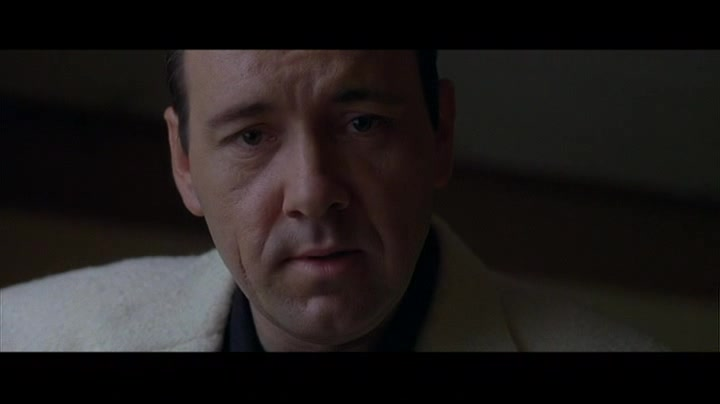
\includegraphics[width=0.49\linewidth]
    {fig/slightLeft.jpg}
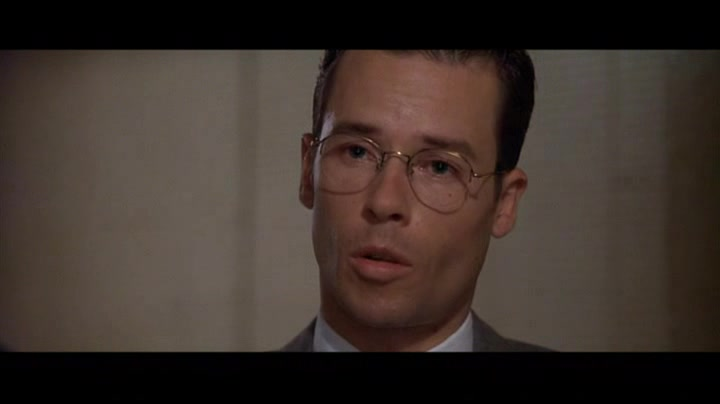
\includegraphics[width=0.49\linewidth]
    {fig/slightRight.jpg}
\end{center}
\caption{These faces might both be classified as centered; however, a human viewer can see the relative left \& right positioning of the faces. These subtleties are better captured using a dynamic grid.}
\label{fig:leftRight}
\end{figure}

\begin{figure}[tb]
\begin{center}
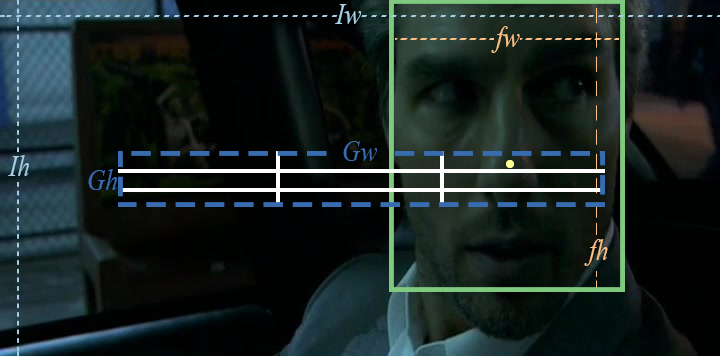
\includegraphics[width=0.75\linewidth]
    {fig/dyGrid.jpg}
\end{center}
\caption{The size of the dynamic grid is based on the size of the face relative to the size of the frame.}
\label{fig:dyGrid}
\end{figure}

\paragraph{The Dynamic Grid}
We use a dynamic grid that  reduces the size of the middle and center sections such that their dimensions are equal to 1/3 of the space in which the facial centroid could occur, see Figure \ref{fig:dyGrid}. The size of the dynamic grid is computed as follows: 
\begin{eqnarray}
  G_{w} &= I_{w} - f_{w} \\
  G_{h} &= I_{h} - f_{h}
\end{eqnarray}

Where $h$ and $w$ represent height and width, respectively, and $G$, $I$, \& $f$ represent Grid, Image, and face. This avoids middle-center convergence, a phenomena where the centroid of large faces converge to the middle-center grid-cell. The dynamic grid  maintains the visual salience of slight position variations (Figure \ref{fig:leftRight}) by preventing middle-center convergence in a principled manner. 
%--------------------------------------------------------------------------------
\begin{figure*}
\begin{center}
\begin{tabular}{c c c c}
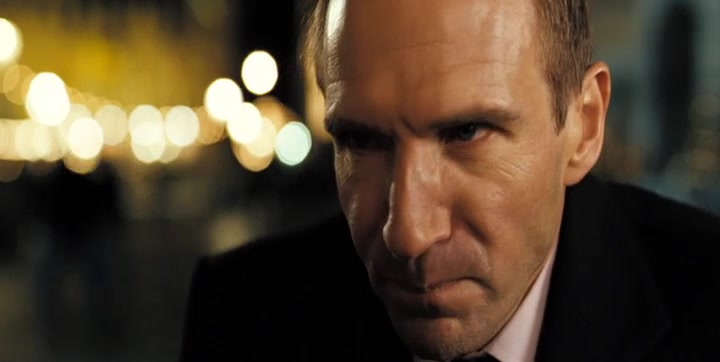
\includegraphics[width=0.22\linewidth]
  {fig/r1.jpg}
& 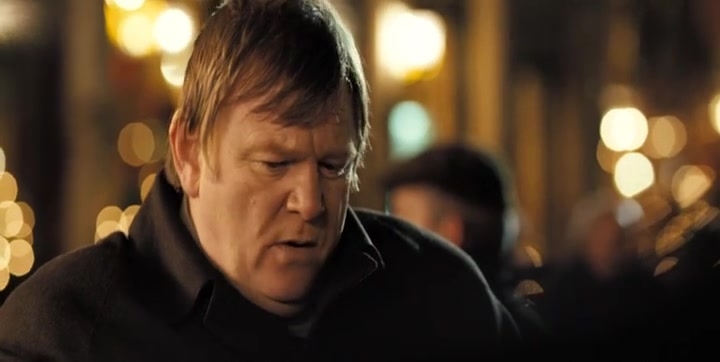
\includegraphics[width=0.22\linewidth]
  {fig/l1.jpg}
& 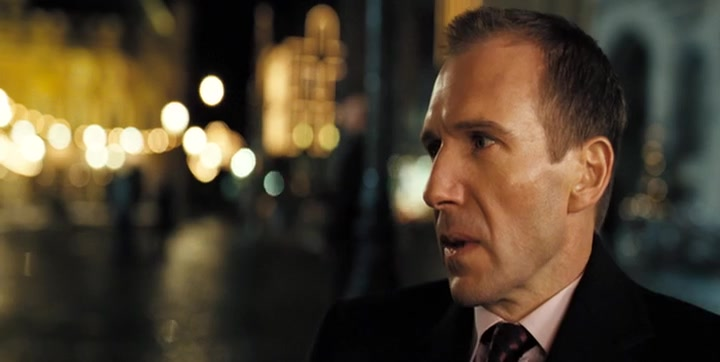
\includegraphics[width=0.22\linewidth]
  {fig/r2.jpg}
& 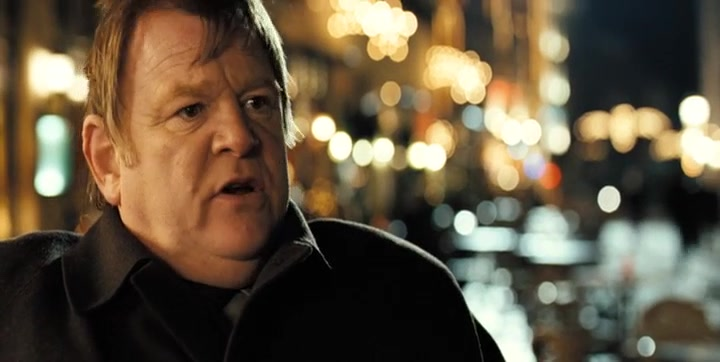
\includegraphics[width=0.22\linewidth]
  {fig/l2.jpg}
\\
\large{1-CU-MR} & \large{1-MCU-ML} & \large{1-CU-MR} & \large{1-MCU-ML} \\
\end{tabular}
\end{center}
\caption{A proper 2-talk sequence maintains the relative left \& right positioning of the actors from shot to shot. Here we have converted the frame sequence into a string: \textit{1-CU-MR, 1-MCU-ML, 1-CU-MR, 1-MCU-ML.}}
\label{fig:2talk}
\end{figure*}

\subsection*{The Sequence}
We define a sequence as a series of frames of arbitrary length. Scenes are then a subset of sequences that fit within the single idea constraint. Defining a sequence as a series of frames with or without scene continuity allows us to search for patterns of frames that are frequently used to construct sequences. One example of this kind of pattern is that used in a 2-actor dialogue. One common construction of a scene in which two actors converse is to place one actor in the right side of the frame and the other actor in the left side of the frame. The frames alternate from showing one actors face to the other, but the relative positioning remains the same, as in Figure \ref{fig:2talk}. \cite{arijon_grammar_1991} defines many possible shot sequences. We use our frame level classifications to convert the problem of sequence pattern discovery and location into an N-Gram analysis problem.

%\begin{figure}
%\begin{center}
%\includegraphics[width=0.45\linewidth]
%    {fig/classes/1-MLS-MC.jpg}
%\includegraphics[width=0.45\linewidth]
%    {fig/classes/2-MCU-TC.jpg}
%\large{1-MLS-MC $\:\:\:\:$}
%\large{$\:\:\:\:\:\:\:\:$ 2-MCU-TC}
%\caption{Frames converted to strings. Left: \textit{1 Face - Medium Long Shot - Middle Center}; Right: \textit{2 Faces - Medium Close-Up - Top Center}. The bounding box for the face in the back of this image is larger than the one for the face in the front. This results in position being classified by her location.}
%\end{center}
%\label{fig:tagExample2}
%\label{fig:tagExample1}
%\end{figure}

%--------------------------------------------------------------------------------
\subsection*{Identifying \& Locating Patterns}
Understanding the visual impact of these sequence structures is best illustrated by the idea of the two person dialogue or '2-talk'. When filming these kinds of sequences, the cinematographer defines the line of interest as the line between the eyes of the two actors, see Figure \ref{fig:lineOfInterest}. The cinematographer places all of the cameras to one side of this line of interest. This significantly reduces the possibility that cameras will appear in each other's image planes. More relevant to our work, it maintains position consistency of the two actors from frame to frame, see Figure \ref{fig:2talk}. 

The 2-talk and other scene and sequence patterns are a key element in cinematographic style. The patterns defined in \cite{arijon_grammar_1991} and other cinematographic textbooks are often what differentiates a professionally filmed motion-picture from what one might see on YouTube. In the frame classification step, we tagged each frame based on its population, zoom, and position. With these tags, we convert a frame into a string as shown in Figure \ref{fig:2talk}. We then define a motion-picture as a string with many such frames. This reduces the problem of visual pattern finding to one of N-Gram analysis.

\begin{figure}[tb]
\begin{center}
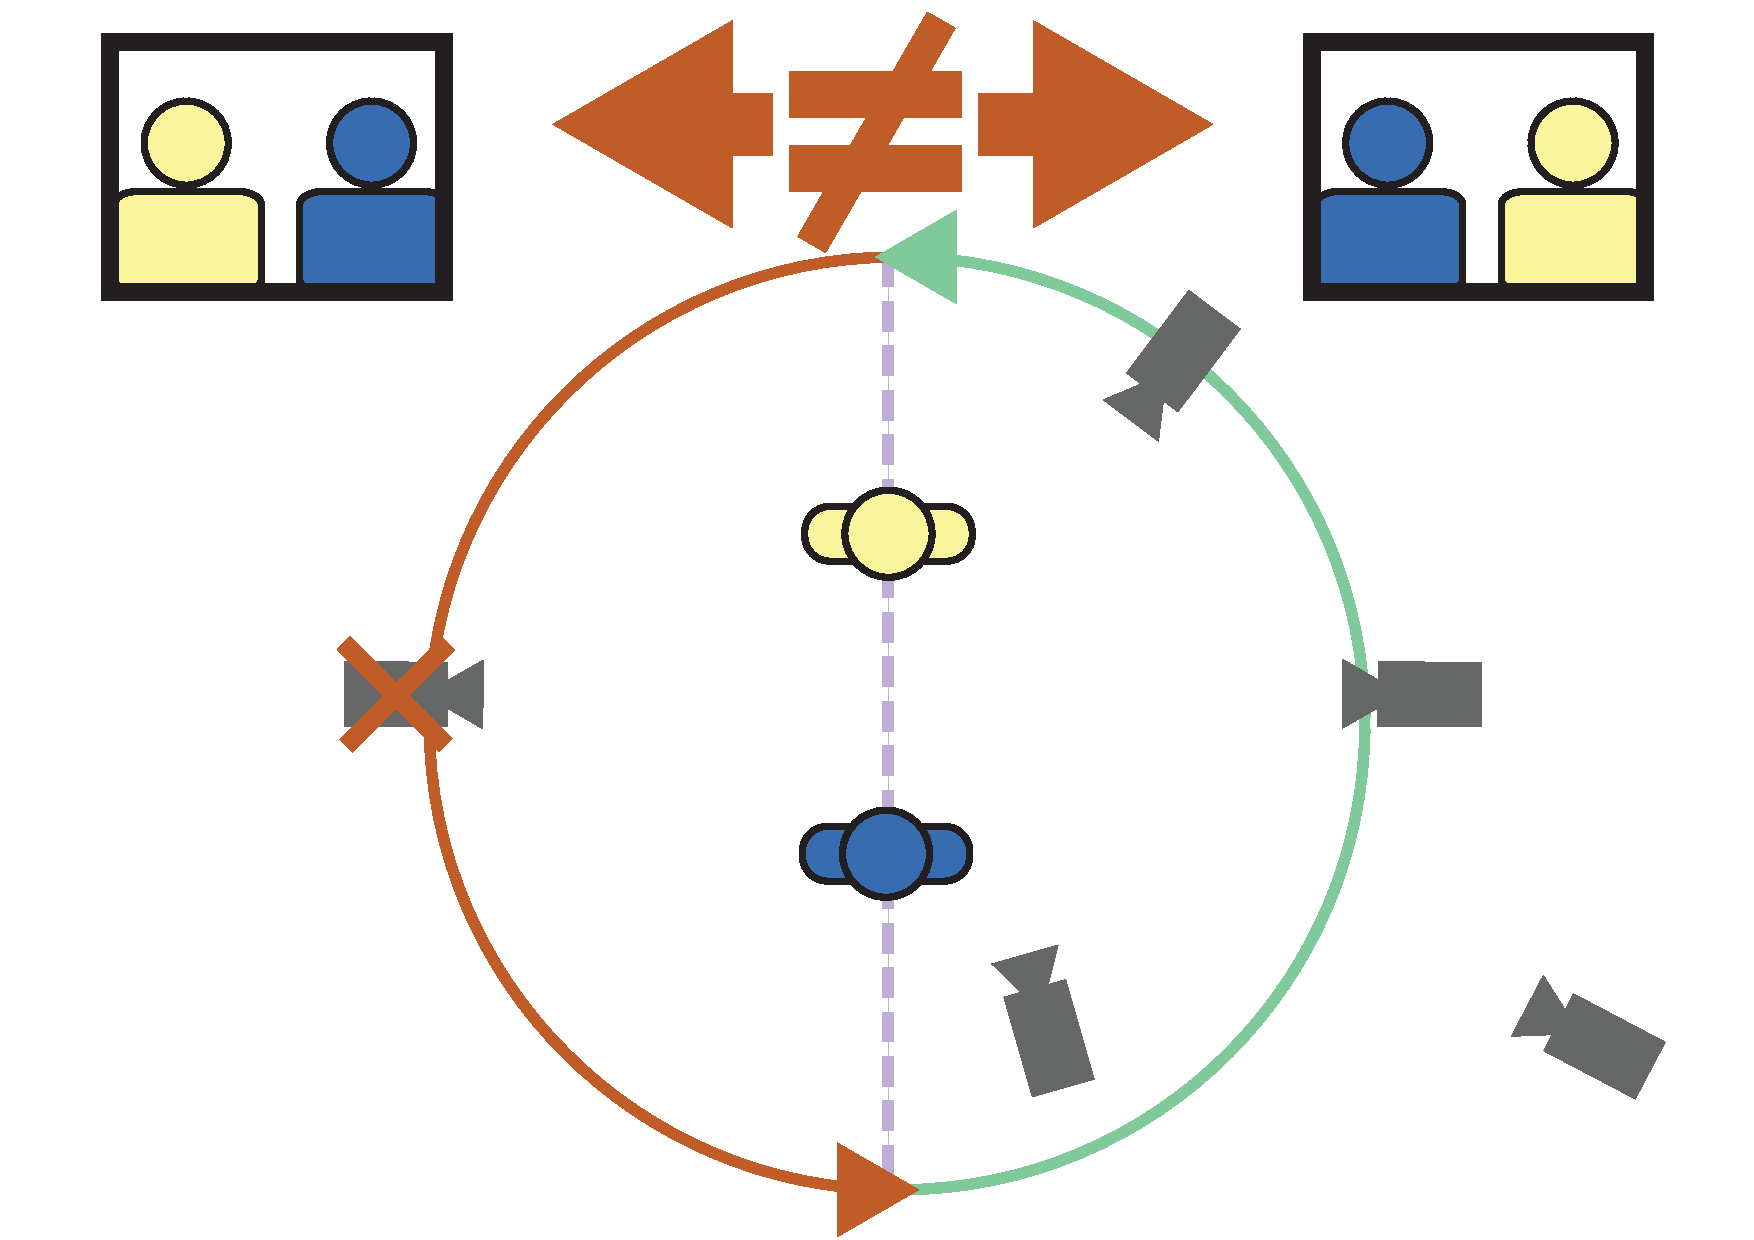
\includegraphics[width=0.5\linewidth]
    {fig/lineOfAction.pdf}
\end{center}
\caption{By placing all cameras on one side of the invisible ``line of interest'' for an entire scene, the relative positioning of actors will remain consistent from shot to shot.}
\label{fig:lineOfInterest}
\end{figure}

%--------------------------------------------------------------------------------
\subsubsection*{N-Gram Analysis}

We reduce our visual pattern finding problem into one of text analysis and use simple N-Gram algorithms to find visual patterns. The primary algorithm we use is most frequent substring. Having defined each movie in a dataset as a string of frame-tags, we pass the set of strings into the algorithm. We also define a minimum length, a maximum length, and a minumum or maximum number of repetitions. The system outputs a list of all patterns that meet our length and repetition critera and their frequency within the dataset. If we have a known pattern, whether selected from a cinematography text or found through our pattern discovery tool, we use simple text-search tools to find which movies contain that pattern and where the pattern occurs. Figures \ref{fig:pat1} shows still-frame examples of a single pattern found in multiple movies.


%--------------------------------------------------------------------------------

\section*{Results}
\begin{figure*}[t!]
\begin{center}
\begin{tabular}{ccccccc}
\large{(A)}
& 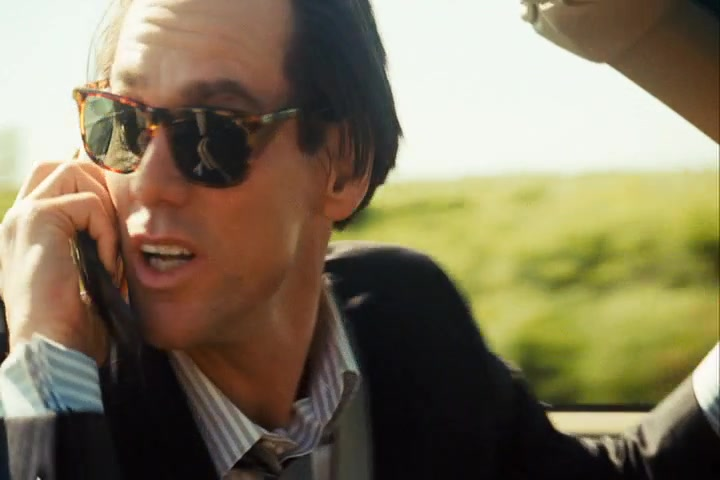
\includegraphics[width=0.12\linewidth]
  {fig/close-ups/01.jpg} 
& 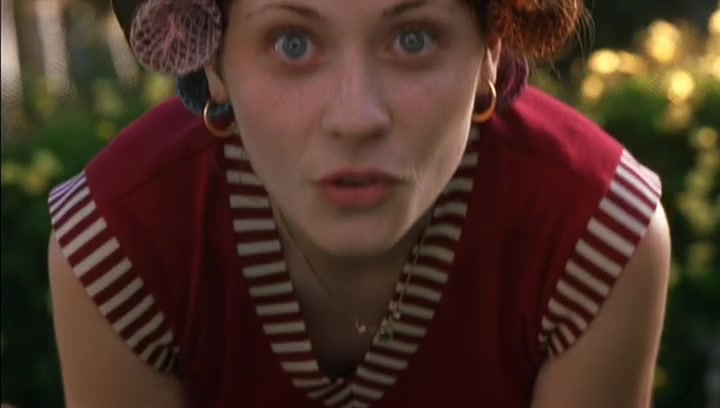
\includegraphics[width=0.12\linewidth]
  {fig/close-ups/02.jpg}  
& 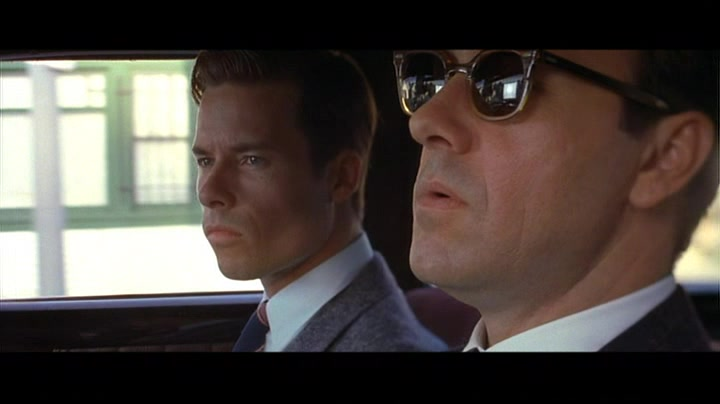
\includegraphics[width=0.12\linewidth]
  {fig/close-ups/10.jpg}   
& 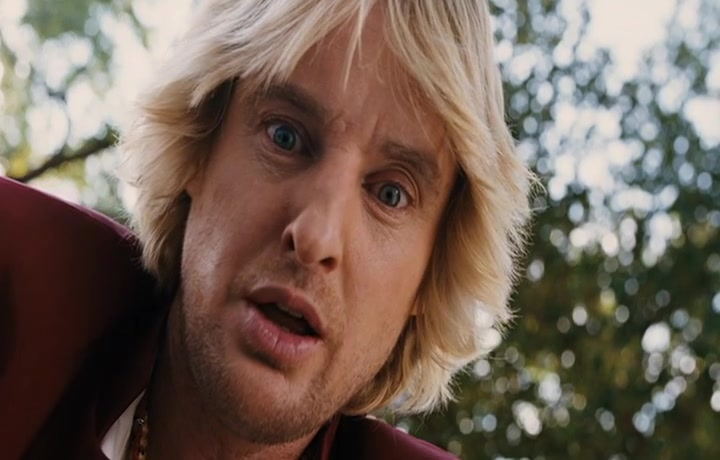
\includegraphics[width=0.12\linewidth]
  {fig/close-ups/15.jpg}
& 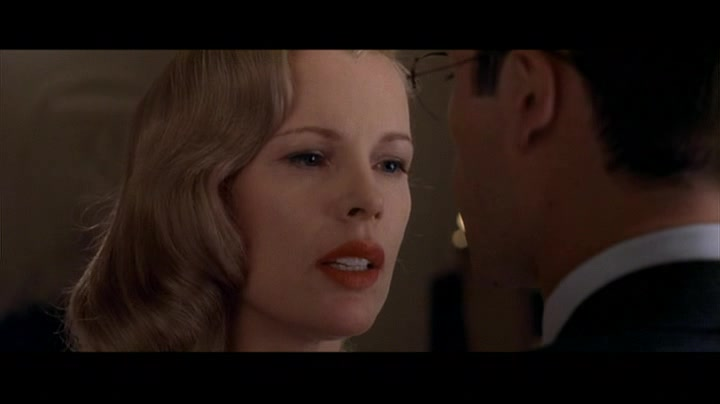
\includegraphics[width=0.12\linewidth]
  {fig/close-ups/05.jpg} 
& 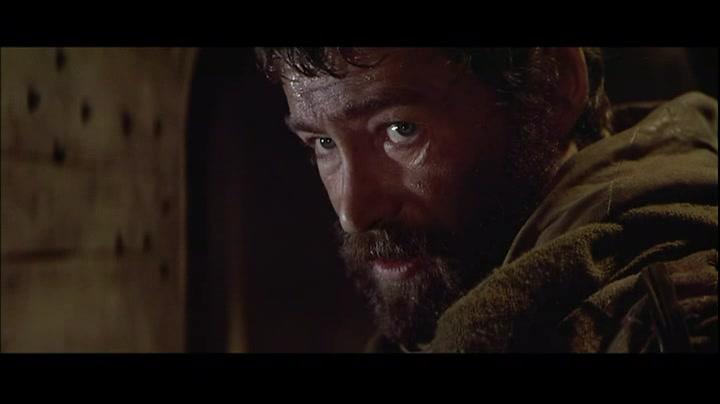
\includegraphics[width=0.12\linewidth]
  {fig/close-ups/06.jpg}  
\\
\end{tabular}
% \bigskip

\begin{tabular}{ccccccc}
\large{(B)}
& 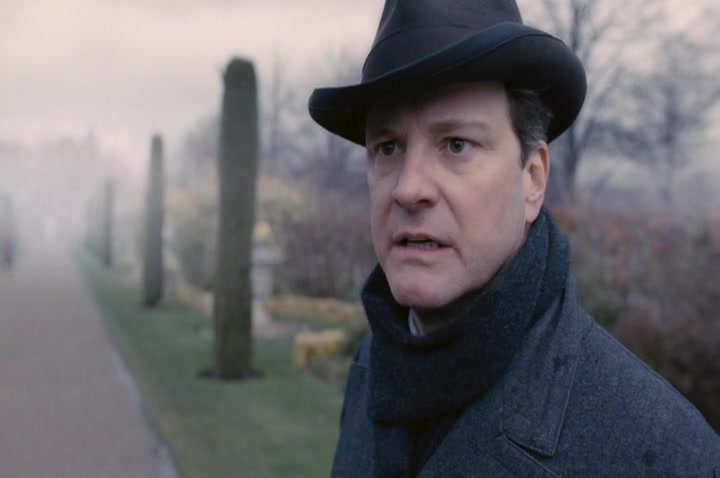
\includegraphics[width=0.12\linewidth]
  {fig/pos/08.jpg} 
& 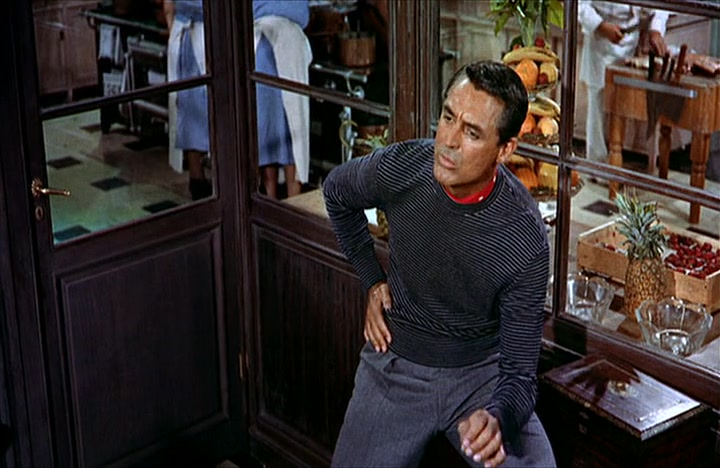
\includegraphics[width=0.12\linewidth]
  {fig/pos/02.jpg}  
& 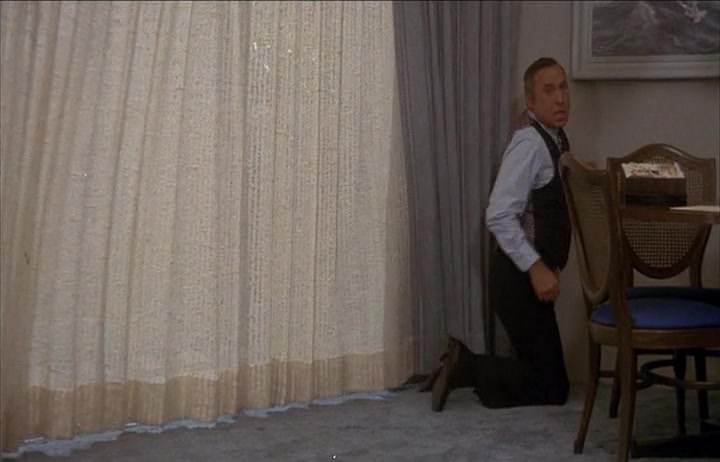
\includegraphics[width=0.12\linewidth]
  {fig/pos/12.jpg}   
& 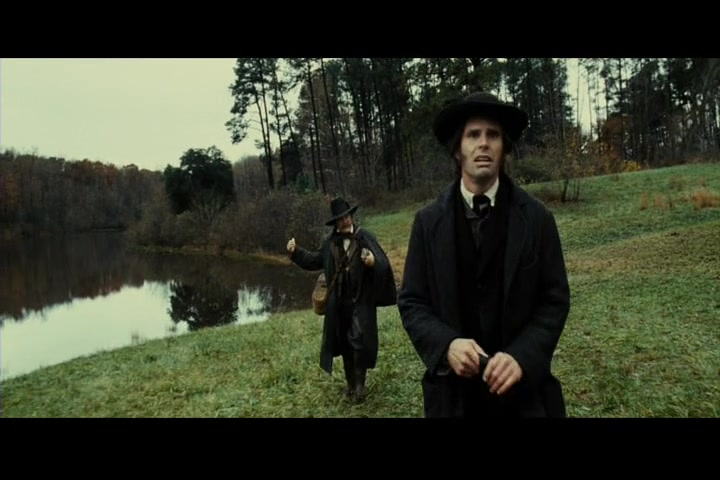
\includegraphics[width=0.12\linewidth]
  {fig/pos/11.jpg}
& 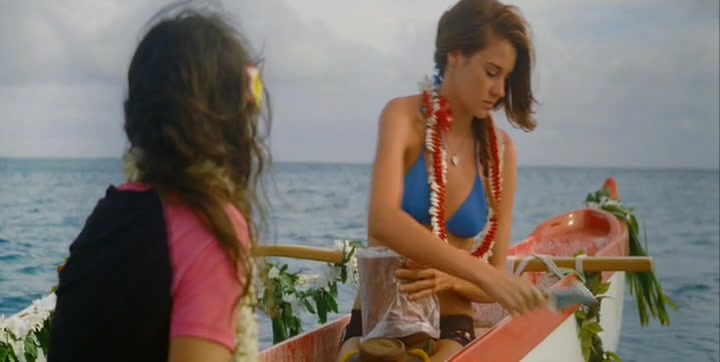
\includegraphics[width=0.12\linewidth]
  {fig/pos/05.jpg}  
& 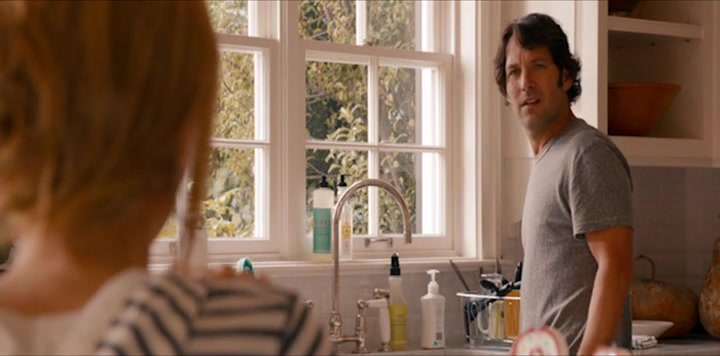
\includegraphics[width=0.12\linewidth]
  {fig/pos/01.jpg}
\\
\end{tabular}
% \bigskip

\begin{tabular}{ccccccc}
\large{(C)}
& 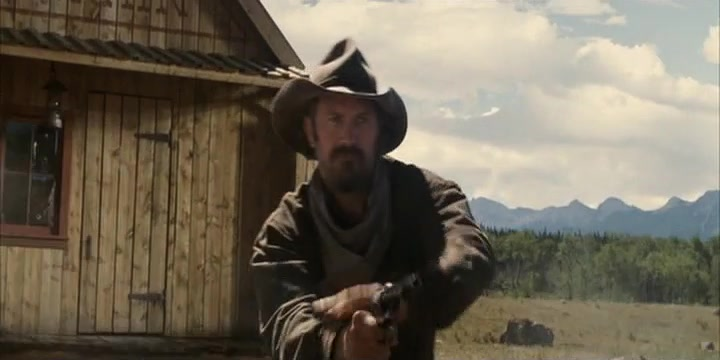
\includegraphics[width=0.12\linewidth]
  {fig/clust/09.jpg} 
& 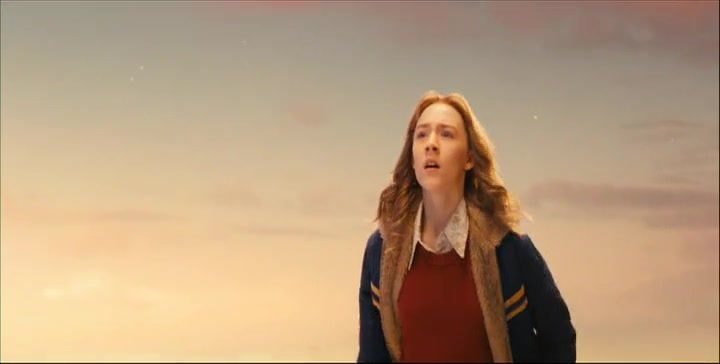
\includegraphics[width=0.12\linewidth]
  {fig/clust/10.jpg}  
& 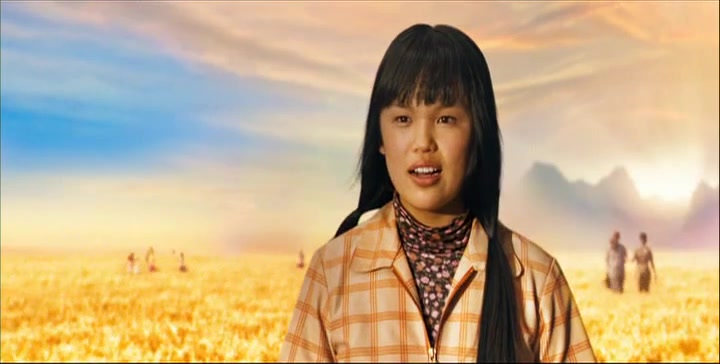
\includegraphics[width=0.12\linewidth]
  {fig/clust/11.jpg}   
% & \includegraphics[width=0.12\linewidth]
%   {fig/clust/12.jpg}
& 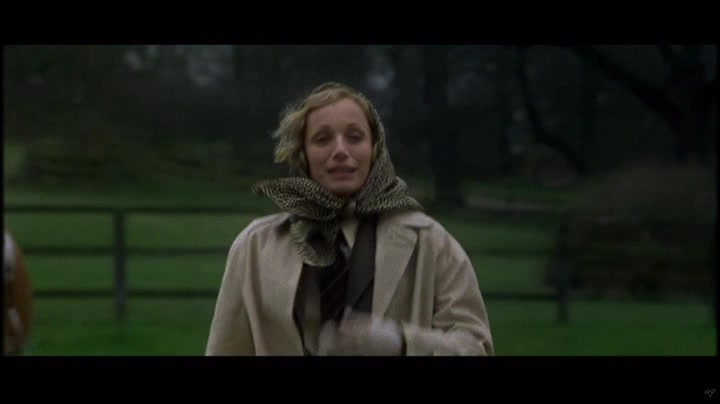
\includegraphics[width=0.12\linewidth]
  {fig/clust/03.jpg} 
& 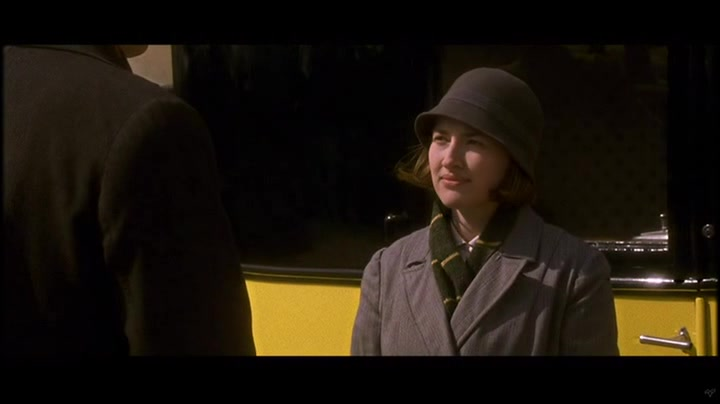
\includegraphics[width=0.12\linewidth]
  {fig/clust/04.jpg}  
& 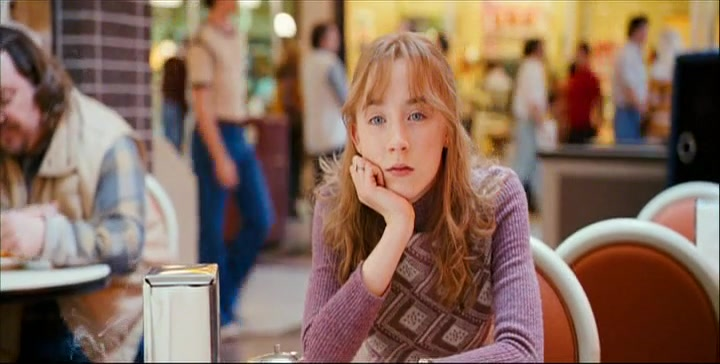
\includegraphics[width=0.12\linewidth]
  {fig/clust/15.jpg}   
% & \includegraphics[width=0.12\linewidth]
%   {fig/clust/16.jpg}
\\
\end{tabular}
\end{center}
   \caption{Example images from our dataset. (A) Close-Ups, (B) Frames with faces in the Top Right, (C) Frames classified as 1-MS-MC}
\label{fig:closeUps}
\label{fig:topRight}
\label{fig:cluster}
\end{figure*}

Figure \ref{fig:closeUps} shows examples of close-ups found in our dataset.
Figure \ref{fig:topRight} shows examples of frames classified as 'Top Right'. Each frame has a face in the upper right region.
Figure \ref{fig:cluster} shows multiple frames that share the same population, zoom, \& position.
%--------------------------------------------------------------------------------

\begin{figure*}
\begin{center}
\begin{tabular}{c c c c c c c}
% \includegraphics[width=0.11\linewidth]
%   {fig/pat1/breach/01.jpg}
% & \includegraphics[width=0.11\linewidth]
%   {fig/pat1/breach/02.jpg}
% & \includegraphics[width=0.11\linewidth]
%   {fig/pat1/breach/03.jpg}
% & \includegraphics[width=0.11\linewidth]
%   {fig/pat1/breach/04.jpg}
% & \includegraphics[width=0.11\linewidth]
%   {fig/pat1/breach/05.jpg}
% & \includegraphics[width=0.11\linewidth]
%   {fig/pat1/breach/06.jpg}
% & \includegraphics[width=0.11\linewidth]
%   {fig/pat1/breach/07.jpg}
% \\

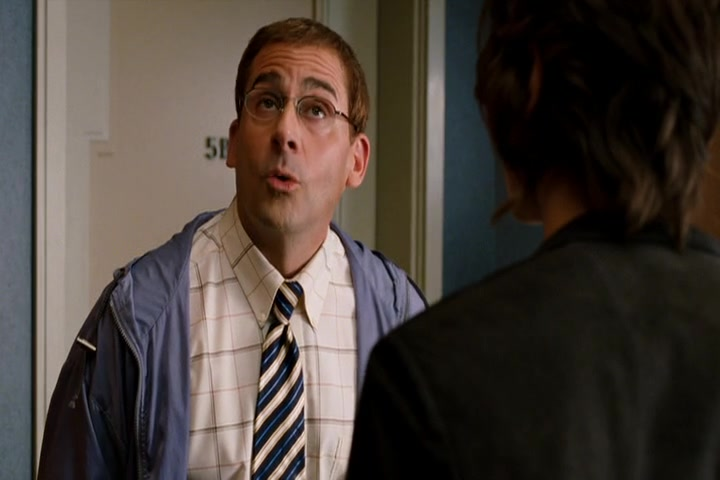
\includegraphics[width=0.11\linewidth]
  {fig/pat1/dinnerForSchmucks/01.jpg}
& 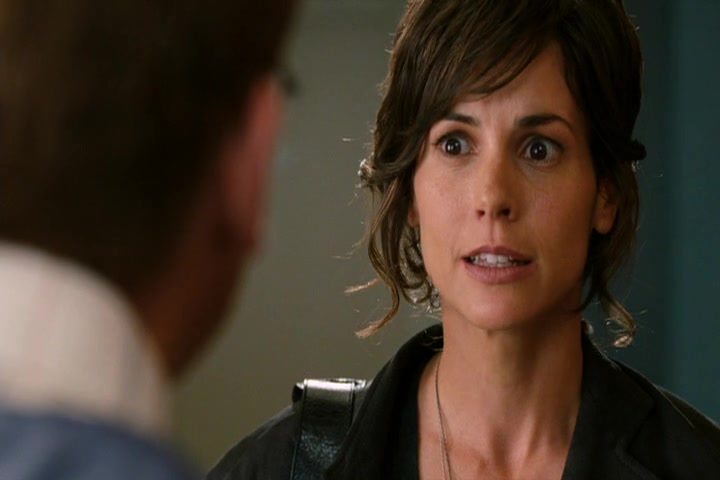
\includegraphics[width=0.11\linewidth]
  {fig/pat1/dinnerForSchmucks/02.jpg}
& 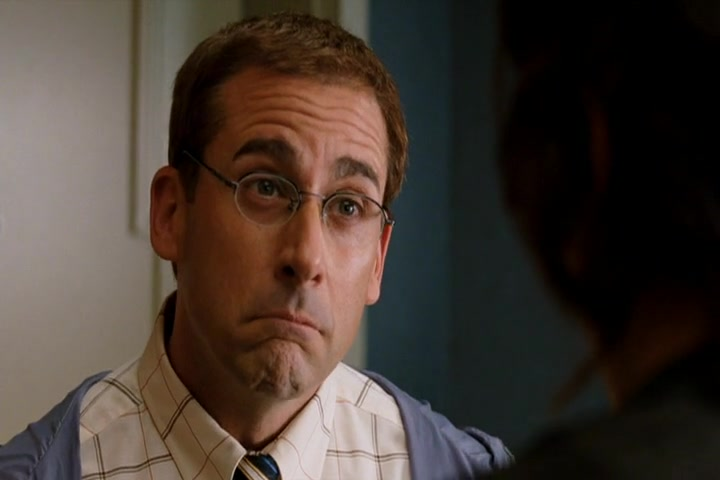
\includegraphics[width=0.11\linewidth]
  {fig/pat1/dinnerForSchmucks/03.jpg}
& 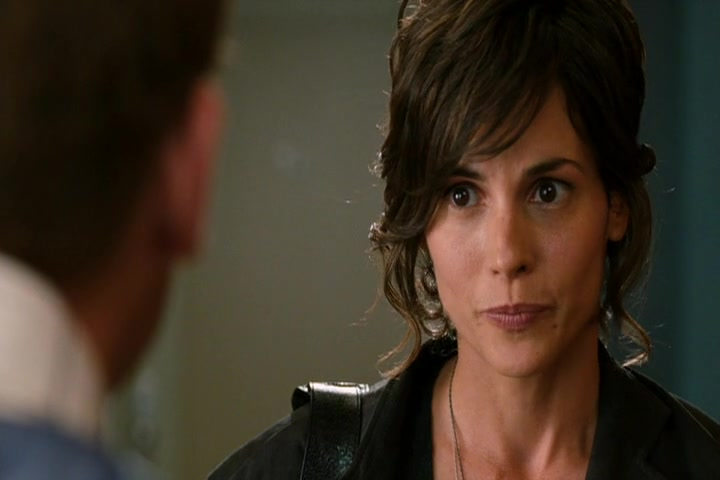
\includegraphics[width=0.11\linewidth]
  {fig/pat1/dinnerForSchmucks/04.jpg}
& 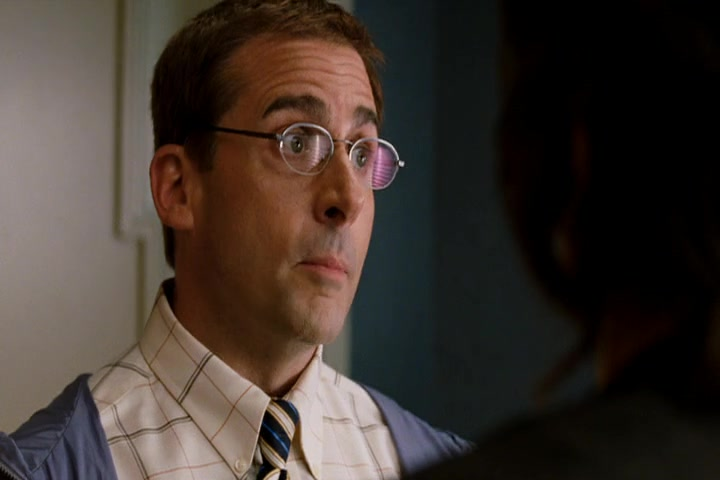
\includegraphics[width=0.11\linewidth]
  {fig/pat1/dinnerForSchmucks/05.jpg}
& 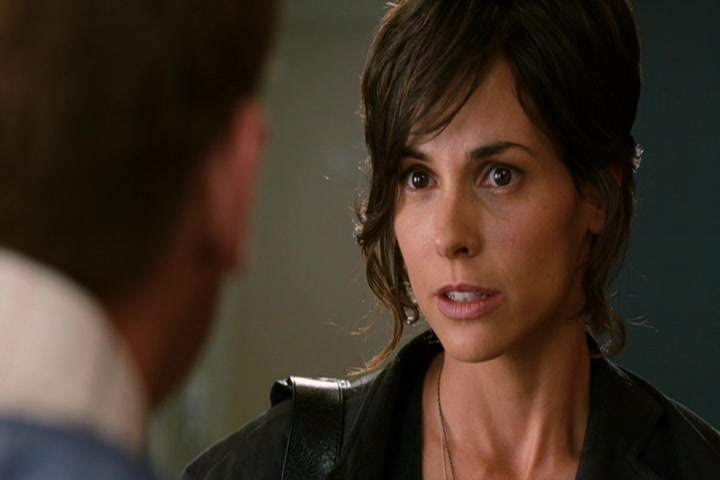
\includegraphics[width=0.11\linewidth]
  {fig/pat1/dinnerForSchmucks/06.jpg}
& 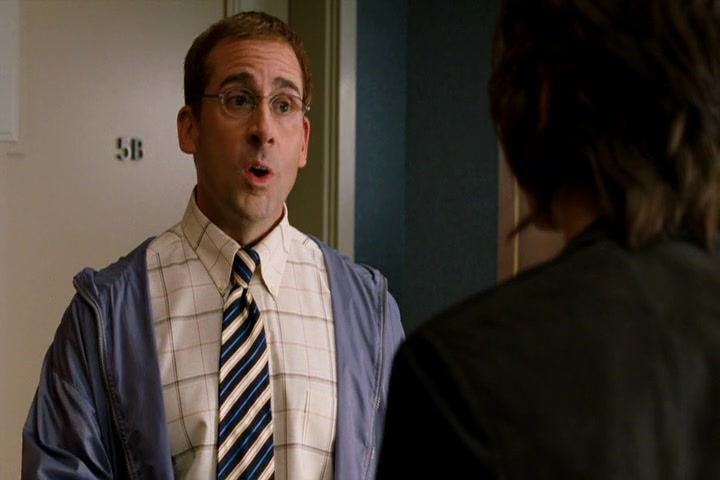
\includegraphics[width=0.11\linewidth]
  {fig/pat1/dinnerForSchmucks/07.jpg}
\\

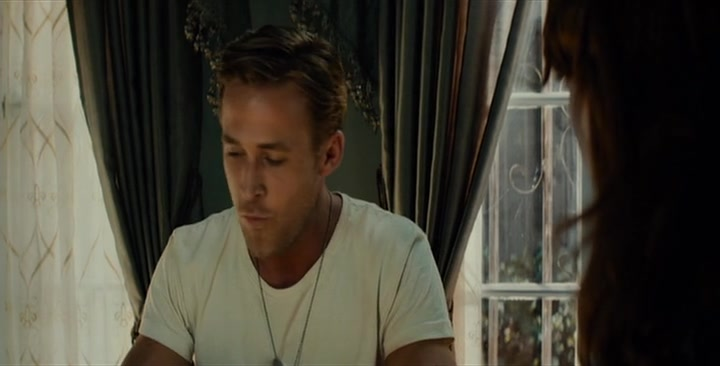
\includegraphics[width=0.11\linewidth]
  {fig/pat1/gangsterSquad/01.jpg}
& 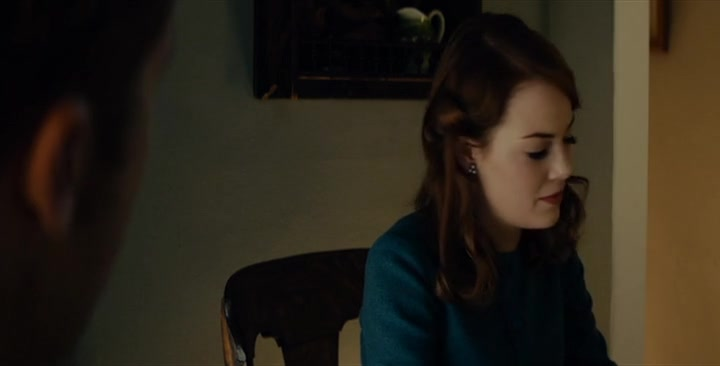
\includegraphics[width=0.11\linewidth]
  {fig/pat1/gangsterSquad/02.jpg}
& 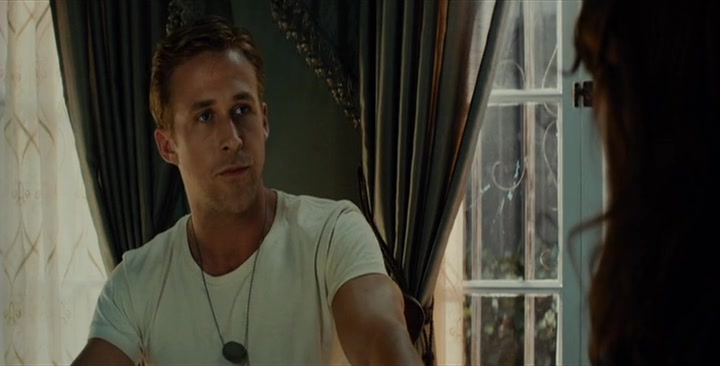
\includegraphics[width=0.11\linewidth]
  {fig/pat1/gangsterSquad/03.jpg}
& 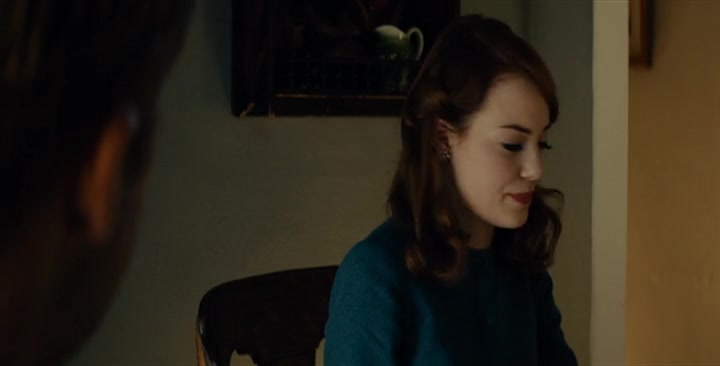
\includegraphics[width=0.11\linewidth]
  {fig/pat1/gangsterSquad/04.jpg}
& 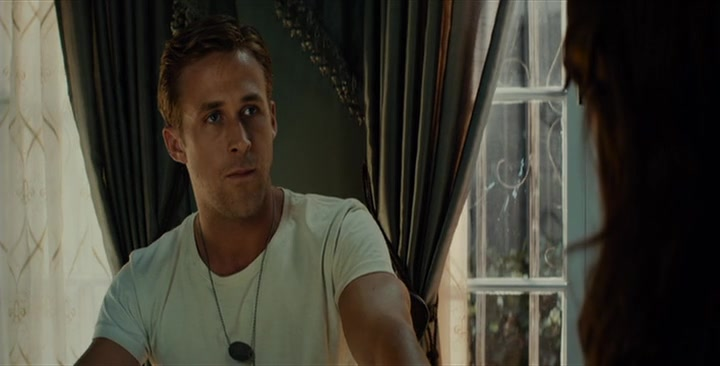
\includegraphics[width=0.11\linewidth]
  {fig/pat1/gangsterSquad/05.jpg}
& 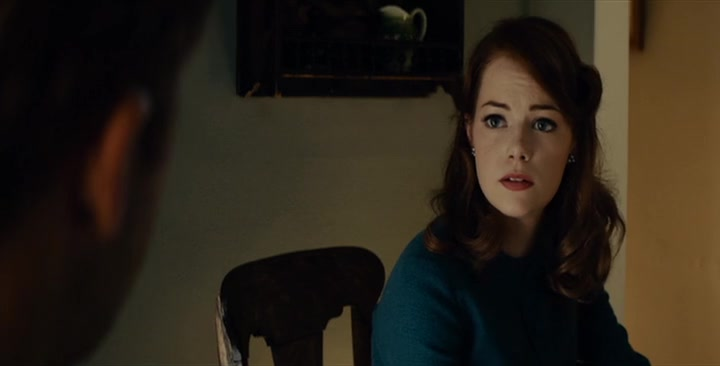
\includegraphics[width=0.11\linewidth]
  {fig/pat1/gangsterSquad/06.jpg}
& 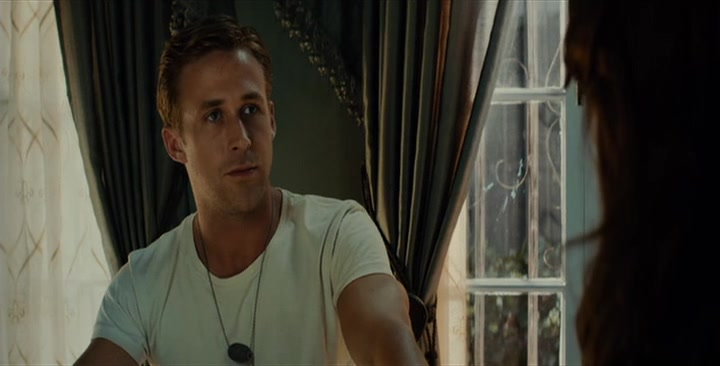
\includegraphics[width=0.11\linewidth]
  {fig/pat1/gangsterSquad/07.jpg}
\\

% \includegraphics[width=0.11\linewidth]
%   {fig/pat1/inBruges/01.jpg}
% & \includegraphics[width=0.11\linewidth]
%   {fig/pat1/inBruges/02.jpg}
% & \includegraphics[width=0.11\linewidth]
%   {fig/pat1/inBruges/03.jpg}
% & \includegraphics[width=0.11\linewidth]
%   {fig/pat1/inBruges/04.jpg}
% & \includegraphics[width=0.11\linewidth]
%   {fig/pat1/inBruges/05.jpg}
% & \includegraphics[width=0.11\linewidth]
%   {fig/pat1/inBruges/06.jpg}
% & \includegraphics[width=0.11\linewidth]
%   {fig/pat1/inBruges/07.jpg}
% \\

% \includegraphics[width=0.11\linewidth]
%   {fig/pat1/theBookOfEli/01.jpg}
% & \includegraphics[width=0.11\linewidth]
%   {fig/pat1/theBookOfEli/02.jpg}
% & \includegraphics[width=0.11\linewidth]
%   {fig/pat1/theBookOfEli/03.jpg}
% & \includegraphics[width=0.11\linewidth]
%   {fig/pat1/theBookOfEli/04.jpg}
% & \includegraphics[width=0.11\linewidth]
%   {fig/pat1/theBookOfEli/05.jpg}
% & \includegraphics[width=0.11\linewidth]
%   {fig/pat1/theBookOfEli/06.jpg}
% & \includegraphics[width=0.11\linewidth]
%   {fig/pat1/theBookOfEli/07.jpg}
% \\

% \includegraphics[width=0.11\linewidth]
%   {fig/pat1/theGirlWithTheDragonTatoo/01.jpg}
% & \includegraphics[width=0.11\linewidth]
%   {fig/pat1/theGirlWithTheDragonTatoo/02.jpg}
% & \includegraphics[width=0.11\linewidth]
%   {fig/pat1/theGirlWithTheDragonTatoo/03.jpg}
% & \includegraphics[width=0.11\linewidth]
%   {fig/pat1/theGirlWithTheDragonTatoo/04.jpg}
% & \includegraphics[width=0.11\linewidth]
%   {fig/pat1/theGirlWithTheDragonTatoo/05.jpg}
% & \includegraphics[width=0.11\linewidth]
%   {fig/pat1/theGirlWithTheDragonTatoo/06.jpg}
% & \includegraphics[width=0.11\linewidth]
%   {fig/pat1/theGirlWithTheDragonTatoo/07.jpg}
% \\

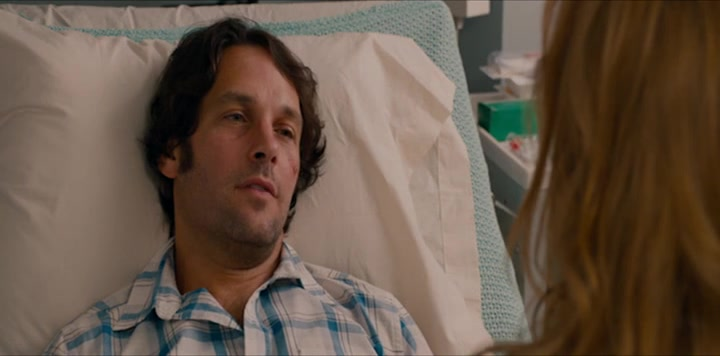
\includegraphics[width=0.11\linewidth]
  {fig/pat1/thisIs40/01.jpg}
& 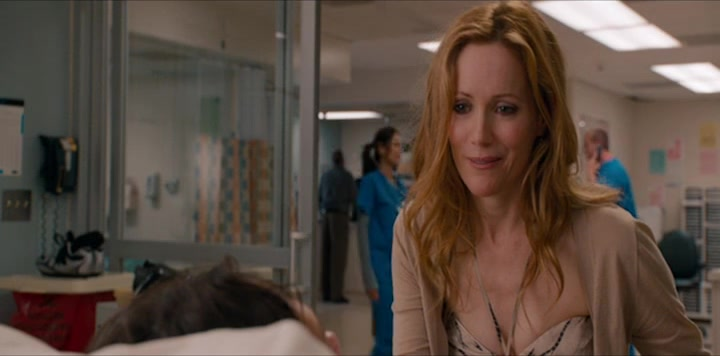
\includegraphics[width=0.11\linewidth]
  {fig/pat1/thisIs40/02.jpg}
& 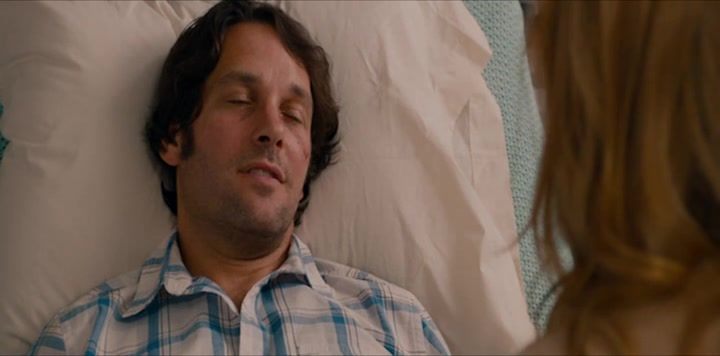
\includegraphics[width=0.11\linewidth]
  {fig/pat1/thisIs40/03.jpg}
& 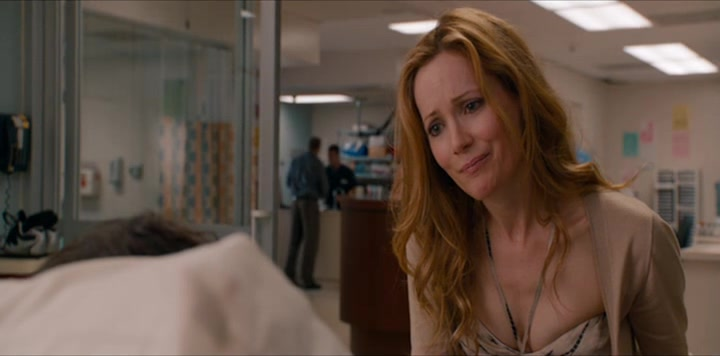
\includegraphics[width=0.11\linewidth]
  {fig/pat1/thisIs40/04.jpg}
& 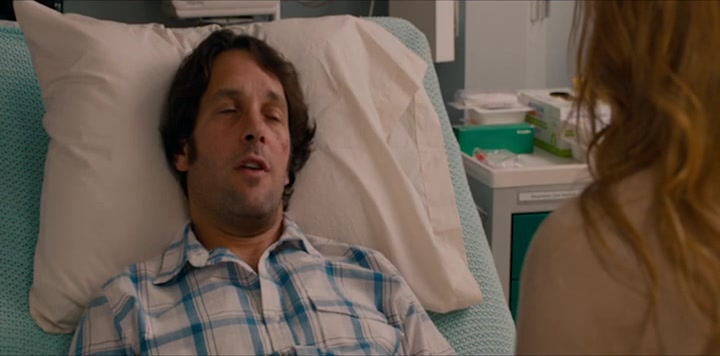
\includegraphics[width=0.11\linewidth]
  {fig/pat1/thisIs40/05.jpg}
& 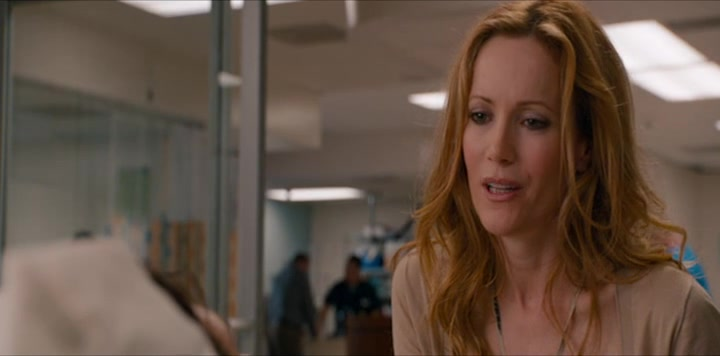
\includegraphics[width=0.11\linewidth]
  {fig/pat1/thisIs40/06.jpg}
& 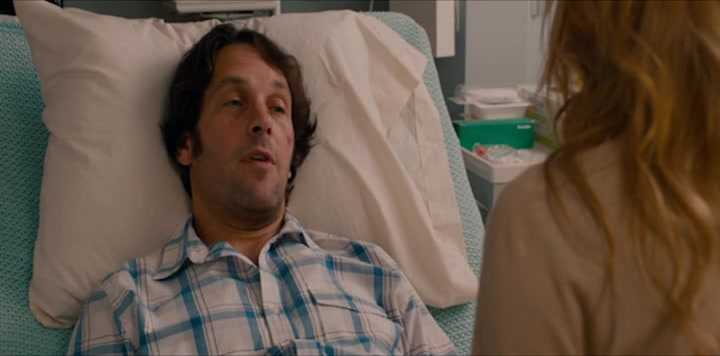
\includegraphics[width=0.11\linewidth]
  {fig/pat1/thisIs40/07.jpg}
\\
\large{1-MCU-L} & \large{1-MCU-R} 
& \large{1-MCU-L} & \large{1-MCU-R} 
& \large{1-MCU-L} & \large{1-MCU-R} 
& \large{1-MCU-L} \\

\end{tabular}
\end{center}
\label{fig:pat1}
\end{figure*}

Figure \ref{fig:pat1} shows still-frame examples of a pattern occurring in several different movies from our dataset. 


\begin{center}
\small{
  \begin{tabular}{ l | r r }
    Movie Clip & Precision \% & Recall \% \\
    \hline
    \textit{ Back To The Future III } &  83.19 &  55.52\\
    \textit{ Breach } &  92.78 &  51.37\\
    \textit{ Broken Flowers } &  92.03 &  4.41\\
    \textit{ Contagion } &  95.98 &  69.09\\
    \textit{ Dazed And Confused } &  80.48 &  11.96\\
    \textit{ Death Proof } &  93.13 &  49.76\\
    \textit{ Dinner For Schmucks } &  73.45 &  23.30\\
    \textit{ Escape From Alcatraz } &  95.16 &  47.91\\
    \textit{ Gosford Park } &  95.27 &  1.94\\
    \textit{ Salt } &  85.42 &  57.66\\
    \textit{ Super 8 } &  84.35 &  49.74\\
    \textbf{ Average } &  \textbf{89.39} &  \textbf{38.63}\\
    \label{tab:shotdetResults}
  \end{tabular}
  }
\end{center}
    
%%%%%%%%%%%%%%%%%%%%%%%%%%%%%%

%--------------------------------------------------------------------------------
\subsection*{Detectors}
%--------------------------------------------------------------------------------
\subsubsection*{Face Detection}
Our current system uses the HeadHunter \cite{mathias_face_2014} detection model as formulated for the Deformable Parts Model \cite{lsvm-pami}. While not quite reaching the performance of the current state-of-the-art, this detector is available off the shelf and can be run on remote clusters with little setup cost. As better face detectors become available, we will incorporate them into our framework.

%--------------------------------------------------------------------------------



\section*{Shot Detection}

Short summary of why we did shot detection (transition from face detection) goes here.

\subsection*{Feature-based approach}

\textbf{Features:} We consider four main types of features to detect cuts in videos. First, we consider changes in luminance (Lum), or mean value of a greyscale image, and color histograms (ColHist) between pairs of frames. Intuitively, luminace and color histograms should change gradually within a shot (low difference values) and drastically across a shot boundary. We also consider the magitude histogram of the optical flow (OptMag) between neighboring frames, and the changes in optical flow between neighboring pairs of frames (OptChange). We consider the absolute magnitude (OptMag), because the optical flow algorithm often produces large vectors when it does not find good matches between neighboring frames. We consider the changes (OptChange) because the optical flow should change less within a shot than it changes between neighboring shots.
\\

\begin{table}[h!]
  \begin{center}
  	\small{
	\begin{tabular}{l|lll}
	Feature   & Precision  & Recall     & F-Measure  \\ \hline
	Lum       & $0.62$ & $0.77$ & $0.69 $ \\
	ColHist   & $0.75$ & $0.78$ & $0.77$ \\
	OptMag    & $0.35$ & $0.82$ & $0.49$ \\
	OptChange & $0.22$ & $0.45$ & $0.30$ \\ \hline
	\end{tabular}
	}
  \end{center}
  \label{table:peakresults}
  \caption{This table shows results for predicting cuts in all videos in our dataset with the peak finding method with each feature (Lum, ColHist, OptMag, and OptChange).}
\end{table} 

\begin{table}[h!]
  \begin{center}
  	\small{
	\begin{tabular}{l|lll}
	Feature   & Precision  & Recall     & F-Measure  \\ \hline
	Lum       & 0.63      & 0.81   & 0.70      \\
	ColHist   & 0.84      & 0.77   & 0.80      \\
	OptMag    & 0.39      & 0.90   & 0.53      \\
	OptChange & 0.15      & 0.54   & 0.23      \\
	\textbf{SVM} & \textbf{0.94} & \textbf{0.84} & \textbf{0.89}\\ \hline
	\end{tabular}
	}
  \end{center}
  \label{table:allresults}
  \caption{This table shows results for predicting cuts in 3 test set videos with the peak finding method with each feature (Lum, ColHist, OptMag, and OptChange) and the SVM that combines the other predictions.}
\end{table} 


\noindent \textbf{Peak finding:} We use each feature to classify cuts by finding peaks in the feature signals. A peak is a local maximum that is at least some threshold higher than the points around it. We include precision, recall and f-measure averaged over all videos for the first 10000 frames in each video in Table~\ref{table:peakresults}.\\

\noindent \textbf{SVM results:} Independently, the color histograms and luminance features scored the best precision and recall. However each feature produced different detections, so we use an SVM to predict whether or not each frame is a cut, given whether or not a peak was predicted for each feature. We randomly selected a training set of 7 videos, and tested on the remaining three videos. Using this method we detect cuts with 0.94 precision , 0.84 recall, 0.89 f-measure. We compare this result to using the peak results alone on the three test videos in Table~\ref{allresults}. 

In the future, we will enter in the difference between the peak and the surrounding frames rather than a binary detect or not detect, as this could further aid the SVM technique.

\subsection*{CNN}

We designed a Convolutional Neural Network for use with shot boundary detection. We computed pairwise differences in luminance; vertical \& horizontal optical flow; \& the red, green, \& blue color channels for every pair of adjacent frames in a video. These differences were passed as as $6 \times h \times w$ matrix where $h = height$ \& $w = width$ of the frames. These arrays were then non-uniformly scaled to $256 \times 256$ pixels to ensure consistency across videos with different aspect ratios. 

Once the $N \times 6 \times 256 \times 256$ arrays had been constructed, they were passed into a 7 layer network, with a network architecture heavily inspired by LeNet \cite{lecun1998gradient}.

Due to time, data, and implementation limitations, we were unable to obtain results from using our architecture, however we plan to continue this work in future research. 


%%% Local Variables:
%%% mode: latex
%%% TeX-master: "finalpaper"
%%% End:


\section*{Summary \& Conclusion}

Short summary and conclusion goes here.

%----------------------------------------------------------------------------------------
%	BIBLIOGRAPHY
%----------------------------------------------------------------------------------------

\bibliographystyle{unsrt}

\bibliography{sample}

%----------------------------------------------------------------------------------------

\end{document}